% chktex-file 12
% chktex-file 36
\section{Perfect matchings, involution products and contraction}\label{sec:matchings}

Throughout, $V$ is a finite set. Working with an arbitrary vertex set lets us restrict to subsets and contract edges without relabelling. Propositions~\ref{prop:moment} and~\ref{prop:invprod} are not used later.

\subsection{Matchings as involutions and union graphs}

A \emph{perfect matching} of $V$ is a fixed-point-free involution $P$ of $V$. We write $P(v)$ for the partner of $v$ and also regard $P$ as the set of its edges $\{v,P(v)\}$. The set of perfect matchings is $\M(V)$, and $\M_n=\M(\{0,1,\dots,2n-1\})$. The symmetric group $S_V$ acts on $\M(V)$ by conjugation, $(\sigma P)(v)=\sigma(P(\sigma^{-1}v))$, so that $\sigma$ sends the edge $\{v,P(v)\}$ to $\{\sigma v,\sigma P(v)\}$. A bijection $V\to V'$ transports matchings by conjugation.

\begin{proposition}\label{prop:count}
Let $|V|=2n$. Then $|\M(V)|=(2n-1)!!$, and $S_V$ acts transitively on $\M(V)$. % chktex 40
\end{proposition}

\begin{proof}
A perfect matching is a permutation of cycle type $2^n$, and conversely. Any two permutations of the same cycle type are conjugate, which gives transitivity. The stabilizer of one matching is the wreath product $S_2\wr S_n$ of order $2^n n!$, so $|\M(V)|=(2n)!/(2^n n!)=(2n-1)!!$. % chktex 40
\end{proof}

For $P,Q\in\M(V)$ the \emph{union graph} $P\cup Q$ is the multigraph on $V$ with the edges of both. Every vertex has degree two, so each connected component is a cycle of even length that alternates between edges of $P$ and of $Q$. An edge common to $P$ and $Q$ is a component with two vertices, a doubled edge, which we count as a cycle of length $2$. Let $\kappa(P\cup Q)$ be the number of components.

\begin{definition}\label{def:H}
$P$ and $Q$ are a \emph{Hamiltonian pair}, written $\Ham(P,Q)$, if $P\cup Q$ is connected. The \emph{Hamiltonicity matrix} $H=H_V$ is the matrix over $\F$ indexed by $\M(V)\times\M(V)$ with $H[P,Q]=[\Ham(P,Q)]$. We write $H_{2n}=H_{\{0,\dots,2n-1\}}$.
\end{definition}

The matrix $H$ is symmetric and $H[\sigma P,\sigma Q]=H[P,Q]$ for $\sigma\in S_V$. On a nonempty vertex set $\Ham(P,Q)$ holds if and only if $\kappa(P\cup Q)=1$. When $|V|=2$ the unique matching $P_0$ satisfies $\Ham(P_0,P_0)$, so $H_2=(1)$. When $|V|>2$ two matchings with a common edge $\{u,v\}$ are never a Hamiltonian pair, because $\{u,v\}$ is then a component of $P\cup Q$ that misses some vertex. In particular $H$ has zero diagonal for $|V|\ge 4$.

\begin{proposition}\label{prop:moment}
Let $|V|=2n\ge2$, $F\in\M(V)$ and $x\ge 1$ a real number. Then
\[
\sum_{P\in\M(V)}x^{\kappa(P\cup F)}\le\prod_{i=0}^{n-1}(x+2i).
\]
\end{proposition}

\begin{proof}
For $|V|=2$ both sides equal $x$. Let $|V|\ge4$, fix $u$, put $u'=F(u)$, $V'=V\setminus\{u,u'\}$ and $\bar F=F/uu'$, and for $P\in\M(V)$ write $\bar P=P/uu'$. The component of $P\cup F$ through $u$ also contains $u'$, and every other component of $P\cup F$ is a component of $\bar P\cup\bar F$. If $P(u)\ne u'$, then $P(u)\in V'$, and the component of $\bar P\cup\bar F$ through $P(u)$ is not among those components, so $\kappa(P\cup F)\le\kappa(\bar P\cup\bar F)$. If $P(u)=u'$, then $\kappa(P\cup F)\le\kappa(\bar P\cup\bar F)+1$. For fixed $c=P(u)$ the map $P\mapsto\bar P$ is injective, since $P(u')=\bar P(c)$ when $c\ne u'$. Since $x\ge1$, each of the $2n-2$ values $c\ne u'$ contributes at most $\Sigma'=\sum_{R\in\M(V')}x^{\kappa(R\cup\bar F)}$, and the value $c=u'$ contributes at most $x\Sigma'$. So the sum is at most $(x+2n-2)\Sigma'$, and induction on $n$ gives the bound.
\end{proof}

\subsection{Cycle structure through the involution product}

For $P,Q\in\M(V)$ put $g=PQ\in S_V$. Since $P$ and $Q$ are involutions, $PgP=QP=g^{-1}$, and the same holds for $Q$. Hence $P$ maps $g$-cycles to $g$-cycles, reversing their direction.

\begin{proposition}\label{prop:invprod}
Let $P,Q\in\M(V)$ and $g=PQ$, with fixed points counted as cycles of length one.
\begin{enumerate}
\item For every $v$, the vertices $v$ and $P(v)$ lie in different $g$-cycles, and so do $v$ and $Q(v)$.
\item A component of $P\cup Q$ with $2k$ vertices is the disjoint union of the $g$-cycle of $v$ and the $g$-cycle of $P(v)$, each of length $k$.
\item The number of cycles of $g$ is $2\kappa(P\cup Q)$.
\item If $|V|=2n$, then $\Ham(P,Q)$ holds if and only if $g$ has exactly two cycles, each of length $n$. For $n\ge2$ this says that $g$ has cycle type $(n,n)$.
\end{enumerate}
\end{proposition}

\begin{proof}
For (i), suppose $g^j(u)=P(u)$ for some $u$ and some $j\ge0$, with $j$ minimal. The case $j=0$ gives $P(u)=u$, and $j=1$ gives $Q(u)=u$. If $j\ge2$, then $g^{j-1}(u)=g^{-1}P(u)=Q(u)=P(gu)$, so $g^{j-2}(gu)=P(gu)$, which contradicts minimality. A negative power $g^{-j}(v)=P(v)$ is the positive power $g^{j}(P(v))=P(P(v))$. The statement for $Q$ is symmetric. Each power of $g$ moves inside one component of $P\cup Q$, and a vertex $w$ of the component of $v$ lies in the $g$-cycle of $v$ or of $P(v)$, according to the parity of its position along the alternating cycle. With (i) this gives (ii), since $P$ maps the $g$-cycle of $v$ bijectively onto the $g$-cycle of $P(v)$. Part (iii) follows from (ii), and (iv) is (iii) together with (ii) for $\kappa=1$. For $n=1$ the product $g$ is the identity with two fixed points.
\end{proof}

By part (ii) of Proposition~\ref{prop:invprod} the permutation $PQ$ has cycle type $(\lambda_1,\lambda_1,\lambda_2,\lambda_2,\dots)$, where $\lambda\vdash n$ lists the half-lengths of the cycles of $P\cup Q$. Diaconis and Holmes call $\lambda$ the distance between $P$ and $Q$, and the distances correspond to the double cosets of $S_2\wr S_n$ in $S_{2n}$~\cite[\S1.5]{DH02}. Part (iv) says that $P$ and $Q$ form a Hamiltonian pair exactly when their distance is $(n)$.

\subsection{Multi-edge contraction}\label{subsec:contraction}

Let $P\in\M(V)$ and let $A\subseteq V$ be nonempty and closed under $P$. Then $P$ is the union of its restriction $P|_A\in\M(A)$ and the matching $P'=P|_{V\setminus A}$ of $V\setminus A$. For $X\in\M(A)$ let $X\cup P'$ be the matching that agrees with $X$ on $A$ and with $P$ off $A$.

Fix $Q\in\M(V)$ and consider the multigraph $Q\cup P'$ on $V$. A vertex of $A$ lies on one edge of $Q$ and on no edge of $P'$, and a vertex of $V\setminus A$ lies on one edge of each. Every component of $Q\cup P'$ is therefore of one of two kinds. It is either a path whose two ends are distinct vertices of $A$, whose inner vertices lie in $V\setminus A$ and whose edges alternate between $Q$ and $P'$, beginning and ending with $Q$, or a cycle inside $V\setminus A$, which we call a \emph{closed cycle}. A $Q$-edge with both ends in $A$ is a path of length one. For $a\in A$ let $Q_A(a)$ be the other end of the path that starts at $a$. Then $Q_A$ is a fixed-point-free involution of $A$, the \emph{exit matching}. It is defined from $Q$ and $P'$ alone, so it does not depend on the matching $X\in\M(A)$, as Figure~\ref{fig:contraction} shows.

\begin{figure}[ht]
\centering
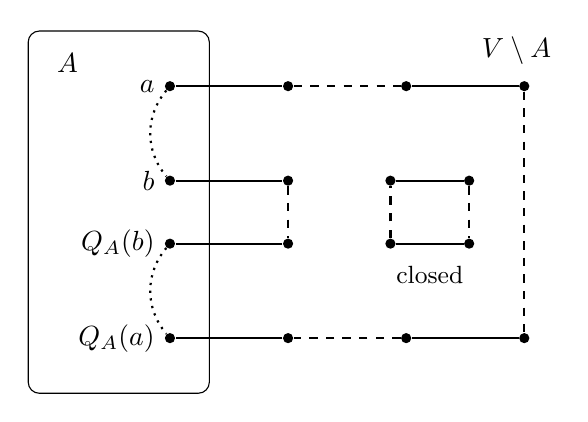
\begin{tikzpicture}[x=1cm,y=1cm,
  v/.style={circle,fill,inner sep=1.3pt},
  qe/.style={thick},
  pe/.style={thick,dashed},
  xe/.style={thick,dotted}]
\draw[rounded corners] (0,-0.3) rectangle (2.3,4.3);
\node at (0.5,3.9) {$A$};
\node at (6.2,4.05) {$V\setminus A$};
\node[v,label=left:{$a$}] (a1) at (1.8,3.6) {};
\node[v,label=left:{$b$}] (b1) at (1.8,2.4) {};
\node[v,label=left:{$Q_A(b)$}] (b2) at (1.8,1.6) {};
\node[v,label=left:{$Q_A(a)$}] (a2) at (1.8,0.4) {};
\node[v] (p1) at (3.3,3.6) {};
\node[v] (p2) at (4.8,3.6) {};
\node[v] (p3) at (6.3,3.6) {};
\node[v] (p4) at (6.3,0.4) {};
\node[v] (p5) at (4.8,0.4) {};
\node[v] (p6) at (3.3,0.4) {};
\node[v] (q1) at (3.3,2.4) {};
\node[v] (q2) at (3.3,1.6) {};
\node[v] (c1) at (4.6,2.4) {};
\node[v] (c2) at (5.6,2.4) {};
\node[v] (c3) at (5.6,1.6) {};
\node[v] (c4) at (4.6,1.6) {};
\draw[qe] (a1)--(p1);
\draw[pe] (p1)--(p2);
\draw[qe] (p2)--(p3);
\draw[pe] (p3)--(p4);
\draw[qe] (p4)--(p5);
\draw[pe] (p5)--(p6);
\draw[qe] (p6)--(a2);
\draw[qe] (b1)--(q1);
\draw[pe] (q1)--(q2);
\draw[qe] (q2)--(b2);
\draw[qe] (c1)--(c2);
\draw[pe] (c2)--(c3);
\draw[qe] (c3)--(c4);
\draw[pe] (c4)--(c1);
\node[font=\small] at (5.1,1.2) {closed};
\draw[xe] (a1) to[bend right=40] (b1);
\draw[xe] (b2) to[bend right=40] (a2);
\end{tikzpicture}
\caption{Solid edges belong to $Q$, dashed edges to $P'$ and dotted edges to a matching $X$ of $A$. The two alternating paths through $V\setminus A$ give the exit matching $Q_A=\{\{a,Q_A(a)\},\{b,Q_A(b)\}\}$, which does not depend on $X$. The $4$-cycle on the right is a closed cycle, so in this picture case (i) of Theorem~\ref{thm:contraction} applies and $H[X\cup P',Q]=0$. Without it, case (ii) gives $H[X\cup P',Q]=H_A[X,Q_A]$.}\label{fig:contraction}
\end{figure}

\begin{theorem}[Contraction]\label{thm:contraction}
Let $P,Q\in\M(V)$, let $A\subseteq V$ be nonempty and closed under $P$, and let $P'=P|_{V\setminus A}$. For every $X\in\M(A)$ the following hold.
\begin{enumerate}
\item If $Q\cup P'$ has a closed cycle, then $H[X\cup P',Q]=0$.
\item Otherwise $H[X\cup P',Q]=H_A[X,Q_A]$.
\end{enumerate}
\end{theorem}

\begin{proof}
In case (i) the vertex set of the closed cycle lies in $V\setminus A$ and is closed under $X\cup P'$ and under $Q$. It misses $A\neq\emptyset$, so $(X\cup P')\cup Q$ is disconnected. In case (ii) every vertex of $V\setminus A$ lies on one of the paths, and each path joins $a$ to $Q_A(a)$. Replacing each path by the edge $\{a,Q_A(a)\}$ turns $(X\cup P')\cup Q$ into $X\cup Q_A$ and preserves connectivity in both directions.
\end{proof}

Cygan, Kratsch and Nederlof prove their factorization of $H$~\cite[Thm.~3.4]{CKN18}, recalled in Section~\ref{subsec:complete}, with a related reduction, which removes two vertices~\cite[App.~A.1, Def.~A.1 and Lemma~A.3]{CKN18}.
